% Frames

% Analysis => Lav uppaal model over roed traad eksempel, lav analysen og kom med resultaterne
\begin{frame}{Analysis of Countermeasures}
\begin{block}{Purpose}
\begin{itemize}
\item To show that under a given set of fault models the implemented countermeasure improves security
\end{itemize}
\end{block}
\begin{block}{Suggestion}
\begin{enumerate}
\item Model the fault model in UPPAAL
\item Model the Java Card program with and without the countermeasure implemented
\item Express properties for the model to verify the protection of the critical code
\end{enumerate}
\end{block}
\end{frame}

\begin{frame}{UPPAAL}{How It Can Be Used}
\begin{itemize}
\item Locations
\begin{itemize}
\item Invariant
\end{itemize}
\item Edges
\begin{itemize}
\item Guard
\item Update
\end{itemize}
\end{itemize}
\begin{center}
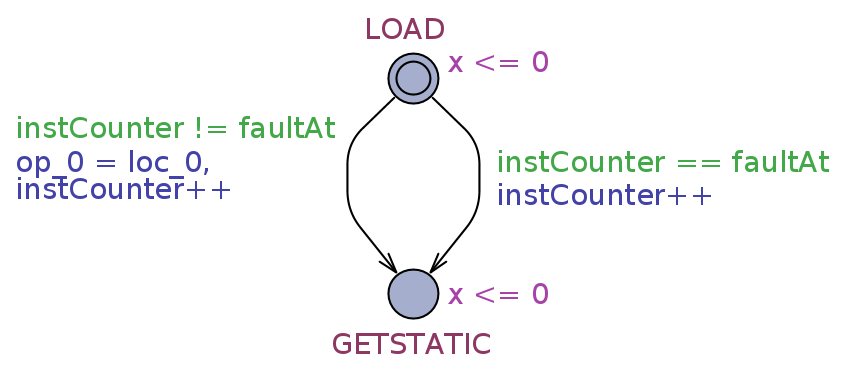
\includegraphics[scale=0.3]{figures/uppaalExample.png}
\end{center}
\end{frame}

\begin{frame}{UPPAAL fault model}
\begin{itemize}
\item At the execution of a random instruction
\item Flip a random bit on all elements on the operand stack
\end{itemize}
\begin{center}
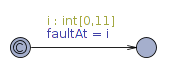
\includegraphics[scale=0.5]{figures/faultmodel.png}
\end{center}
\end{frame}

\begin{frame}{UPPAAL example code}{Without Countermeasures}
\begin{adjustwidth}{-2cm}{-2cm}
\begin{center}
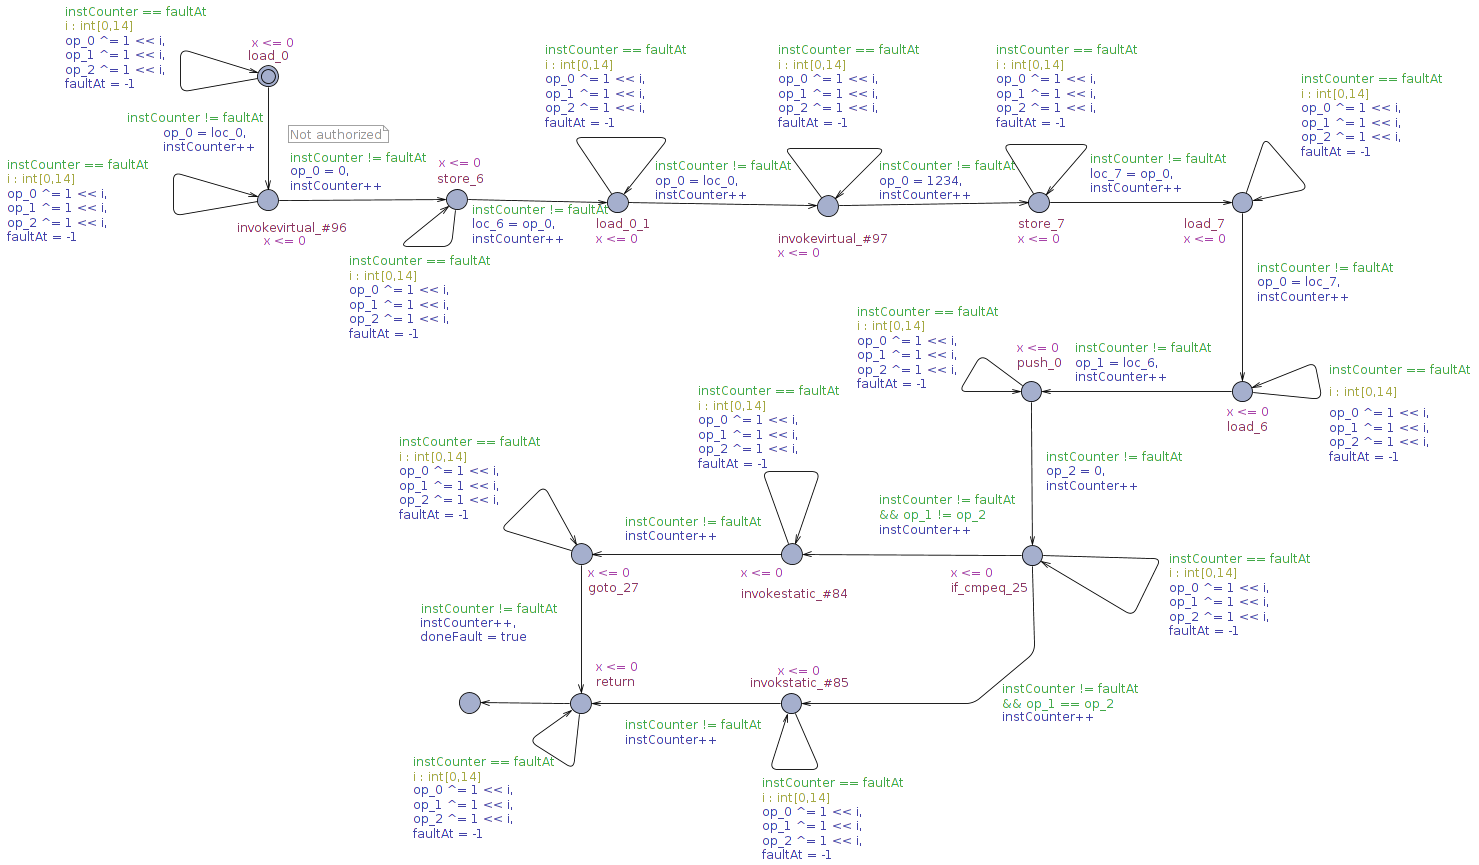
\includegraphics[scale=0.22]{figures/tinyJCL.png}
\end{center}
\end{adjustwidth}
\end{frame}

\begin{frame}{UPPAAL example code}{Without Countermeasures}
\begin{center}
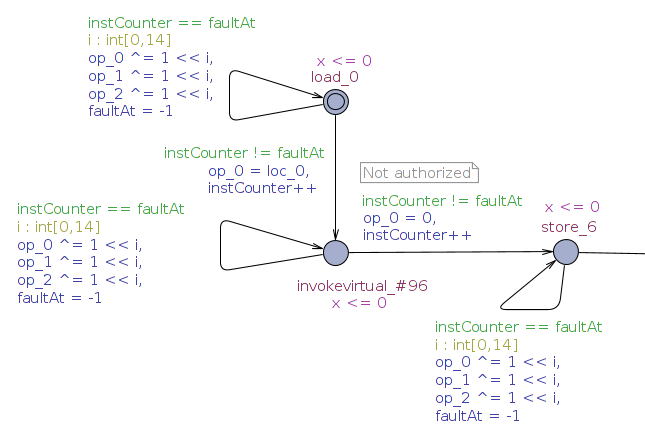
\includegraphics[scale=0.4]{figures/tinyJCLexplained.png}
\end{center}
\end{frame}

\begin{frame}{UPPAAL example code}{Operand Stack Invariant}
\begin{adjustwidth}{-2cm}{-2cm}
\begin{center}
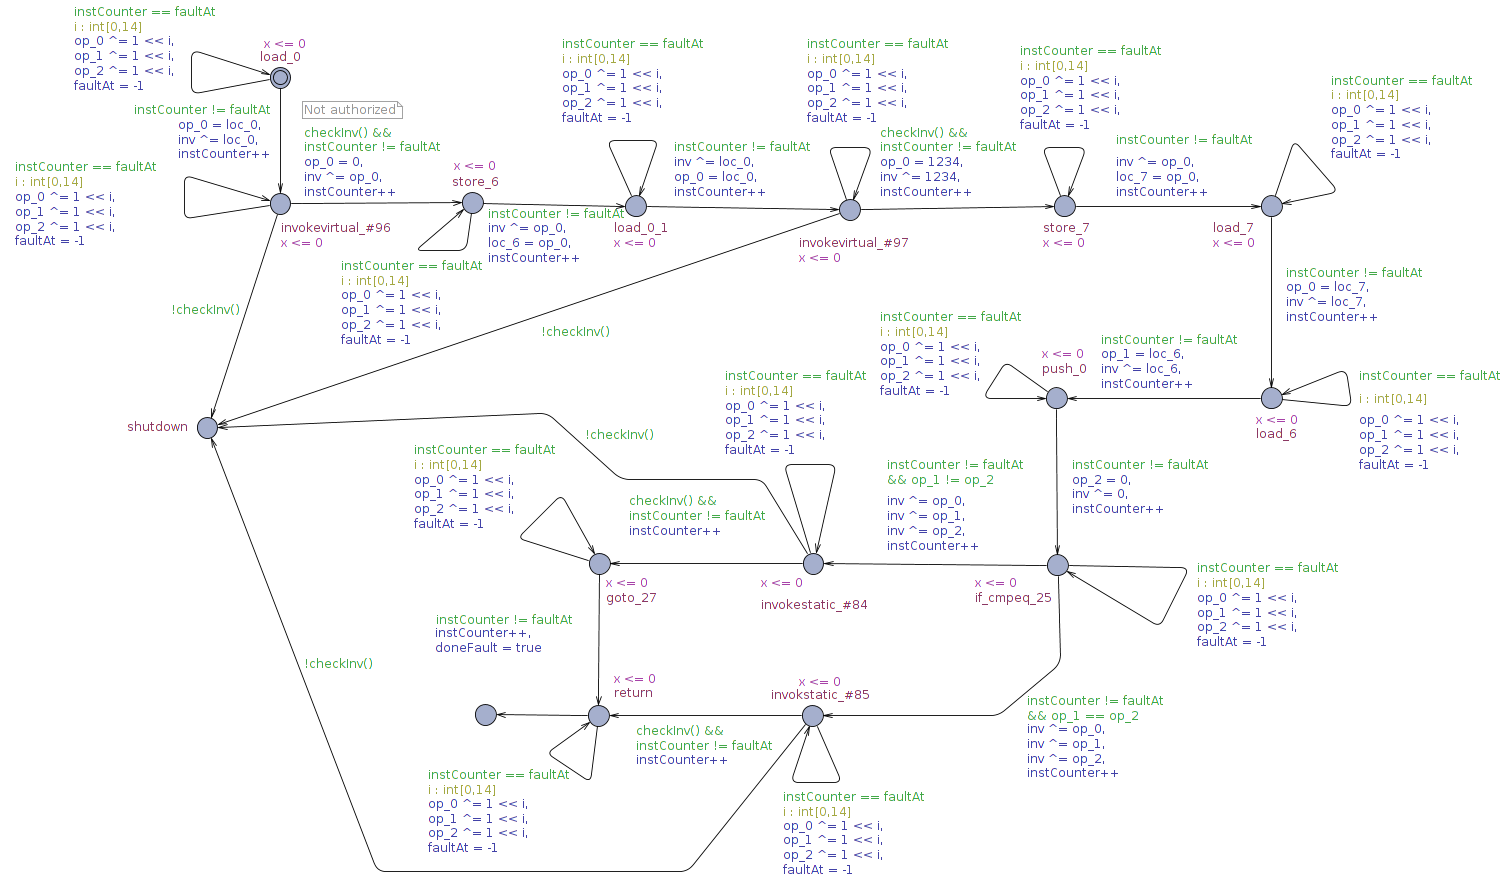
\includegraphics[scale=0.22]{figures/tinyJCLinvariant.png}
\end{center}
\end{adjustwidth}
\end{frame}

\begin{frame}{UPPAAL example code}{Operand Stack Invariant}
\begin{adjustwidth}{-2cm}{-2cm}
\begin{center}
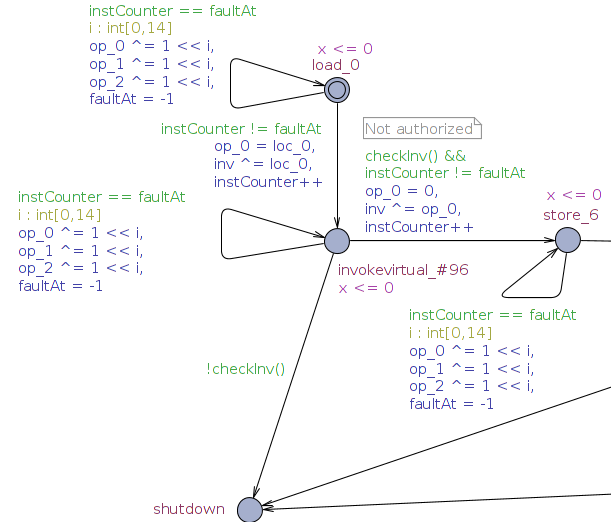
\includegraphics[scale=0.35]{figures/tinyJCLinvariantexplained.png}
\end{center}
\end{adjustwidth}
\end{frame}

\begin{frame}{UPPAAL example code}{Code Duplication}
\begin{adjustwidth}{-2cm}{-2cm}
\begin{center}
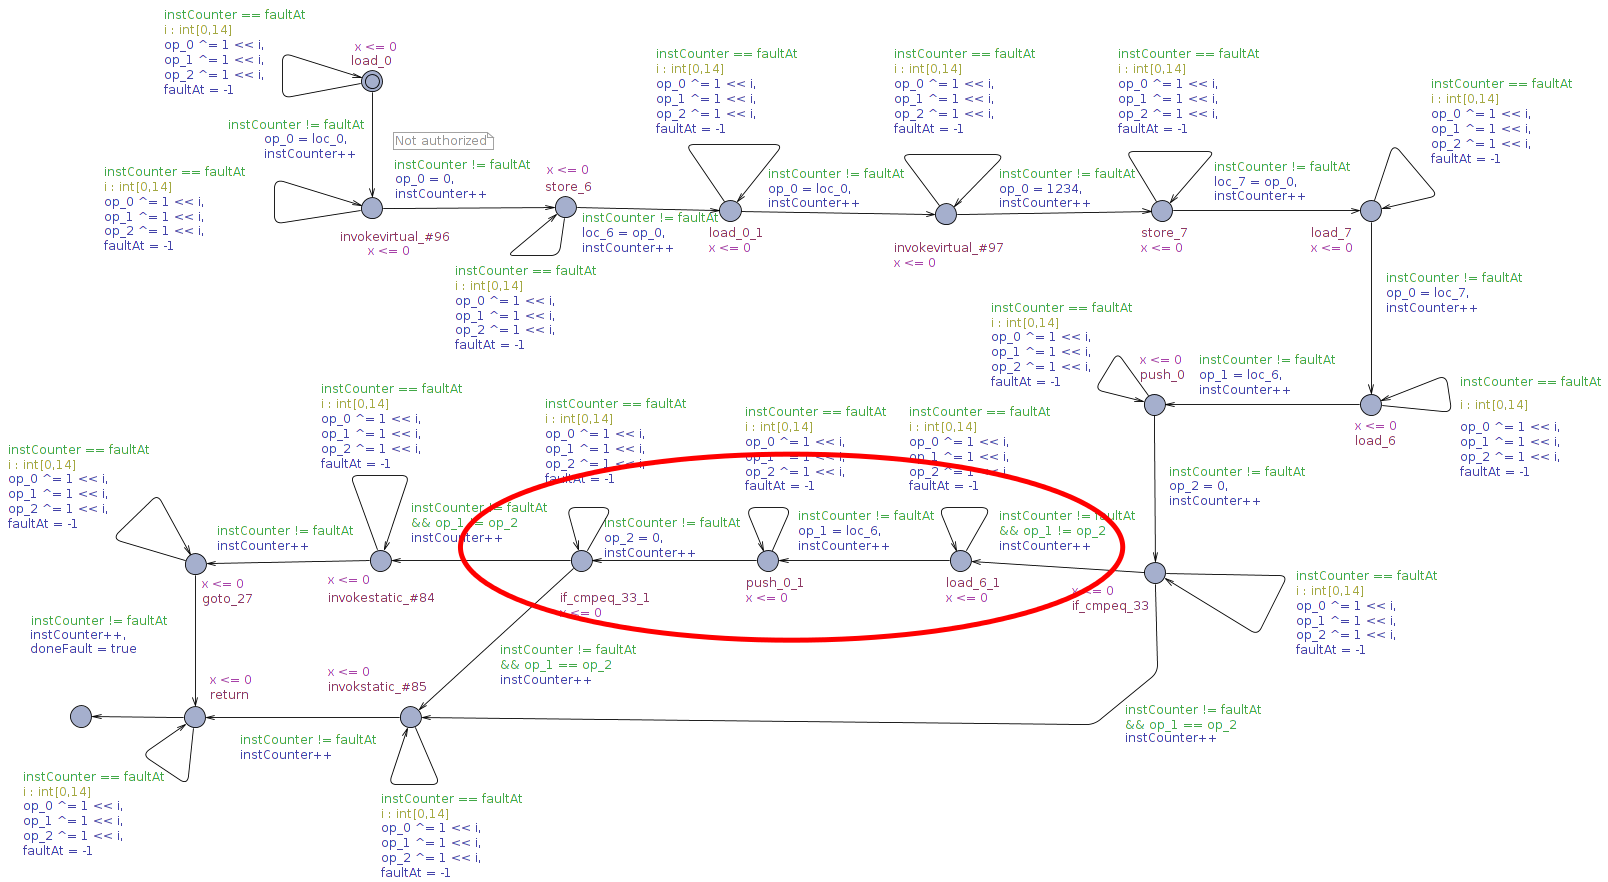
\includegraphics[scale=0.22]{figures/tinyJCLdup.png}
\end{center}
\end{adjustwidth}
\end{frame}

\begin{frame}{UPPAAL example code}{Results}
% \begin{block}{Query}
% \begin{itemize}
% \item \texttt{E[<=3; 1000000] (max : doneFault)}
% \end{itemize}
% \end{block}
\begin{block}{Results}
\begin{table}[]
\centering
\begin{tabular}{l|l|l}
No Countermeasure & Stack Invariant & Code Duplication \\ \hline
16.6 \%           & 0 \%            & 8.3 \%          
\end{tabular}
\end{table}
\end{block}
% Show the query
% Every attack on the operand stack is caught
\end{frame}

% Fut. Work => Recap af hvad man kunne arbejde videre med, forklaret på en anden maade end det i rapporten.
\begin{frame}{Future Work}{Two Identified Directions}
\begin{block}{Analysis of Countermeasures}
\begin{itemize}
\item Be able to parse an annotated program
\item Be able to parse a semantics and a fault model
\item Output a UPPAAL model to visualise the effectiveness of the countermeasures in question
\end{itemize}
\end{block}
\begin{block}{Implementation of Countermeasures}
\begin{itemize}
\item Parse a program and implement countermeasures
\item Annotated code to indicate which parts to protect and the level of security
\item Trade-off between countermeasure effectiveness and computational overhead
\end{itemize}
\end{block}
\end{frame}

%%% Local Variables:
%%% mode: plain-tex
%%% TeX-master: "AAUsimpletheme"
%%% End:

